\documentclass[12pt]{article}

\usepackage[utf8]{inputenc}
\usepackage{datetime}
\usepackage{amsthm}
\usepackage{amsmath}
\usepackage{amssymb}
\usepackage{enumitem}
\usepackage[USenglish]{babel}
\usepackage{matlab-prettifier}
\usepackage{graphicx}
\usepackage[makeroom]{cancel}
\usepackage{afterpage}
\usepackage{capt-of}

\DeclareMathOperator*{\argmin}{arg\,min}
\DeclareMathOperator*{\argmax}{arg\,max}

\newcommand\independent{\protect\mathpalette{\protect\independenT}{\perp}}
\def\independenT#1#2{\mathrel{\rlap{$#1#2$}\mkern2mu{#1#2}}}

\newtheoremstyle{colon}{\topsep}{\topsep}{}{}{\bfseries}{:}{ }{}
\theoremstyle{colon}
\newtheorem{exercise}{Exercise}
\newtheorem*{answer}{Answer}

\title{ORFE 525: Statistical Learning and \\ Nonparametric Estimation \\ Homework 5}
\author{Zachary Hervieux-Moore}

\newdate{date}{27}{04}{2017}
\date{\displaydate{date}}

\begin{document}

\maketitle

\clearpage

\begin{exercise}
  We all know that AlphaGo developed by Google DeepMind defeated the human champion Lee Sedol last year. This is a huge improvement in the development of artificial intelligence because professional Go players were thought to be invicible before. This year, AlphaGo is coming back and a full length three game match will be played against Jie Ke, currently ranked number one in the world, at the Future of Go Summit in Wuzhen on 23 to 27 May, 2017.

  In this problem, we will develop our own AlphaGo to play the Go game. Consider the Go board as an undirected Graph $G = (V,E)$ with $V=\{1,\mathellipsis,19\} \times \{1, \mathellipsis,19\}$ and $N = \lvert V \rvert = 19 \times 19$, nodes $n \in V$ representing the vertices on the board and edges $e \in E$ connecting vertically and horizontally neighboring points. We can denote a position as the vector $c \in \{\text{Black}, \text{White}, \text{Empty}\}^N$ and similarly the final territory outcome of the game as $s \in \{+1, -1\}^N$. For convenience we score from the point of view of Black so elements of $s$ representing Black territory are valued +1 and elements representing white territory are valued -1.

  Go players will note that we are adopting the Chinese method of scoring empty as well as occupied intersections. The distribution we wish to model is $\mathbb{P}_\theta(s,c)$, that is, the distribution over final territory outcomes given the current position.

  In order to predict the final territory outcome, we consider the following graphical model:
  \begin{gather*}
    \mathbb{P}_\theta(s | c) = \frac{1}{Z(c,\theta)} \exp \left( \sum_{(j,k) \in E} w(c_j, c_k) s_j s_k + h(c_j) s_j + h(c_k) s_k \right)
  \end{gather*}
  Where the edges, again, connect all the neighboring nodes on the board. We assume the parameters $w(c_j, c_k)$, $h(c_j)$ are symmetric and only have five possible parameters, i.e.,
  \begin{itemize}
    \item $w_{\text{chains}} = w(\text{Black}, \text{Black}) = w(\text{White}, \text{White})$
    \item $w_{\text{winter-chains}} = w(\text{Black}, \text{White}) = w(\text{White}, \text{Black})$
    \item $w_{\text{chain-empty}} = w(\text{Empty}, \text{White}) = w(\text{Empty}, \text{Black})$
    \item $w_{\text{empty}} = w(\text{Empty}, \text{Empty})$
    \item $h_{\text{stone}} = h(\text{Black}) = -h(\text{White})$
  \end{itemize}
  and $h(\text{Empty}) = 0$ by symmetry.

  We use $\theta$ to denote the above five parameters. Given the training set $\{c_i, s_i\}_{i=1}^K$, we aim to estimate the parameter $\theta$ through MLE. We consider the loss function
  \begin{gather*}
    \mathcal{L}_n (\theta) = -\frac{1}{K} \sum_{i=1}^K \log \mathbb{P}_\theta(s_i | c_i)
  \end{gather*}
  \begin{enumerate}[label=\arabic*)]
    \item The file \texttt{2014Games.zip} contains the Go games in 2014 played by professional players. There are two folders inside: \texttt{Games\_Move80} and \texttt{Games\_Final}. In the folder \texttt{Games\_Move80}, it contains 300 games after move 80 and in the folder \texttt{Games\_Final}, it contains the final positions of the corresponding games in \texttt{Games\_Move80}. In the folders, each game is stored in a text file with a $19 \times 19$ matrix representing the Go board. Here we use +1 for ``Black'', -1 for ``White'', and 0 for ``Empty''.

      We use the games after the move 80 in the folder \texttt{Games\_Move80} as our $c_i$'s. Now we define the final territoy $s_i$'s. You may notice that in the folder \texttt{Games\_Final}, the final position board, denoted by $\tilde{s}_i$, contains many empties. We need to determine each if empty belonds to white or black, i.e., decide the values as $\{+1, -1\}$ in the empty positions. Let $\tilde{s} \in \{\text{Black}, \text{White}, \text{Empty}\}^N$ be the positions in the final move. Given an empty node $(j_0, k_0)$, let
      \begin{gather*}
        j_{\max} = \argmin \{j > j_0 : \tilde{s}_{j, k_0} \neq \text{Empty} \} \\
        j_{\min} = \argmax \{j < j_0 : \tilde{s}_{j, k_0} \neq \text{Empty} \} \\
        k_{\max} = \argmin \{k > k_0 : \tilde{s}_{j_0, k} \neq \text{Empty} \} \\
        k_{\min} = \argmax \{k < k_0 : \tilde{s}_{j_0, k} \neq \text{Empty} \} \\
      \end{gather*}
      Therefore, we give the value to $s_{j_0, k_0}$ by the stone on the set $\mathcal{I}(j_0,k_0) = \{(j_0, k_{\max}), (j_0, k_{\min}), (j_{\max}, k_0), (j_{\min}, k_0)\}$,
      \begin{gather*}
        s_{j_0, k_0} = +1; \text{if} \quad \# \{ \tilde{s}_{jk} = \text{Black} : (j,k) \in \mathcal{I}(j_0, k_0) \} \\
        > \# \{ \tilde{s}_{jk} = \text{White} : (j,k) \in \mathcal{I}(j_0, k_0) \}, \\
        s_{j_0, k_0} = -1; \text{if} \quad \# \{ \tilde{s}_{jk} = \text{Black} : (j,k) \in \mathcal{I}(j_0, k_0) \} \\
        \leq \# \{ \tilde{s}_{jk} = \text{White} : (j,k) \in \mathcal{I}(j_0, k_0) \}
      \end{gather*}
      This means we decide the value of the empty by comparing the number of whites and blacks on the cross extended from this empty. If the extended line attaches the boundary, we just delete this index and compare. For example, if the set $\{j > j_0 : \tilde{s}_{j, k_0} \neq \text{Empty} \} = \emptyset$, we delete $(j_{\max}, k_0)$ from $\mathcal{I}(j_0, k_0)$ and similar for other cases.

      Generate the training dataset $\{c_i, s_i\}_{i=1}^K$ following the above rule.

    \item We aim to use gradient descent algorithm to minimize $\mathcal{L}_n(\theta)$. The problem is that the normalizer $Z(c, \theta)$ is hard to compute, not to mention its gradient. However, we have a smart method to compute the gradient of $\mathcal{L}_n(\theta)$. We denote $f(s,c,\theta) = \sum_{(j,k) \in E} w(c_j, c_k) s_j s_k + h(c_j) s_j + h(c_k) s_k$. Prove that
      \begin{gather*}
        \frac{\partial \mathcal{L}_n (\theta)}{\partial \theta} = \frac{1}{K} \sum_{i=1}^K \mathbb{E}_{s \sim \mathbb{P}_\theta(s | c_i)} \big[ \frac{\partial f(s, c_i, \theta)}{\partial \theta} \big] - \frac{1}{K} \sum_{i=1}^K \frac{\partial f(s, c_i, \theta)}{\partial \theta}
      \end{gather*}
      Therefore, we can use the function \texttt{IsingSampler} in \texttt{R} to sample i.i.d. data from Ising model $\mathbb{P}_\theta(s|c)$ to estimate the expectation term. You can set the number of iterations in \texttt{IsingSampler} as \texttt{nIter = 20} or even smaller at the begging of gradient descent. Estimate the parameter $\hat{\theta}$ using the MLE and gradient descent.

    \item Now we can create the policy network similar to the real AlphaGo. To compare our estimator with AlphaGo, we use the real games between AlphaGo and Lee Sedol as our testing dataset.

      We use the 2nd game (AlphaGo wins) and the 4th game (Lee Sedol wins) as the testing dataset. You can find the two games in the file \texttt{AlphaGo-vs-Lee.zip}. We still use the position after the 80th move $c$ as the input and you can compute the expectation of final territory $\mathbb{E}_{s \sim \mathbb{P}_{\hat{\theta}}(s | c)} [ s_j ]$ for each $j \in V$. Predict the result by calculated the expected score $\sum_{j \in V} \mathbb{E}[s_j] - 3.75$ (Black's handicap is called Komi). If the score is positive, then Blacks wins and if negative, White wins. Compare your prediction with the true result. Plot your expected stone placement after the 80th move with the true result.
  \end{enumerate}
\end{exercise}

\begin{answer}
  \leavevmode
  \begin{enumerate}[label=\arabic*)]
    \item Code used for this question is appended below.

    \item The estimator calculated was
      \begin{gather*}
        \hat{\theta} = (-916.63, -36437.33, -50113.47, -121359.15, 136258.34)
      \end{gather*}
      Proof of the gradient goes as follow
      \begin{align*}
        \mathcal{L}_n (\theta) &= -\frac{1}{K} \sum_{i=1}^K \log \left(\frac{1}{Z(c_i,\theta)} e^{f(s_i,c_i,\theta)} \right) \\
        \mathcal{L}_n (\theta) &=  \frac{1}{K} \sum_{i=1}^K \log Z(c_i,\theta) - \frac{1}{K} \sum_{i=1}^K f(s_i,c_i,\theta) \\
        \implies \frac{\partial \mathcal{L}_n (\theta)}{\partial \theta} &= \frac{1}{K} \sum_{i=1}^K \frac{1}{Z(c_i,\theta)} \frac{ \partial Z(c_i,\theta)}{\partial \theta} - \frac{1}{K} \sum_{i=1}^K \frac{\partial f(s_i,c_i,\theta)}{\partial \theta}
      \end{align*}
      We have the first term, and so now we show that $\frac{1}{Z(c_i,\theta)} \frac{ \partial Z(c_i,\theta)}{\partial \theta} = \mathbb{E}_{s \sim \mathbb{P}_\theta(s | c_i)} \big[ \frac{\partial f(s, c_i, \theta)}{\partial \theta} \big]$. We have
      \begin{align*}
        \frac{1}{Z(c_i,\theta)} \frac{ \partial Z(c_i,\theta)}{\partial \theta} &= \frac{1}{Z(c_i,\theta)} \frac{\partial}{\partial \theta} \int Z(c_i, \theta) \mathbb{P}_{\theta}(s | c_i) ds \\
        &= \frac{1}{Z(c_i,\theta)} \int \frac{\partial}{\partial \theta} e^{f(s, c_i, \theta)}ds \\
        &= \int \frac{\partial}{\partial \theta} f(s, c_i, \theta) \frac{e^{f(s, c_i, \theta)}}{Z(c_i,\theta)} ds \\
        &= \int \frac{\partial}{\partial \theta} f(s, c_i, \theta) \mathbb{P}_{\theta}(s | c_i)ds \\
        &= \mathbb{E}_{s \sim \mathbb{P}_\theta(s | c_i)} \big[ \frac{\partial f(s, c_i, \theta)}{\partial \theta} \big]
      \end{align*}
      Which shows the result.

    \item Game 2 predictions of the final stones is shown in Figure 1 and the actual board in Figure 2. The predicted winner was white and the actual winner was white. Game 4 predictions of the final stones is shown in Figure 3 and the actual board in Figure 4. Predicted winner was white and the actual winner was white.
      \begin{center}
        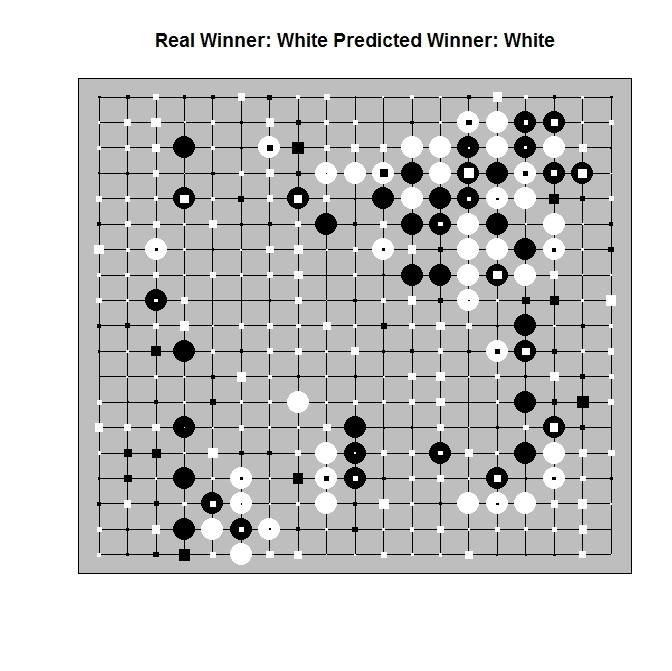
\includegraphics[width=0.9\textwidth]{game_2_prediction.jpg}
        \captionof{figure}{Game 2: Predicted Stone Placement}
      \end{center}

      \begin{center}
        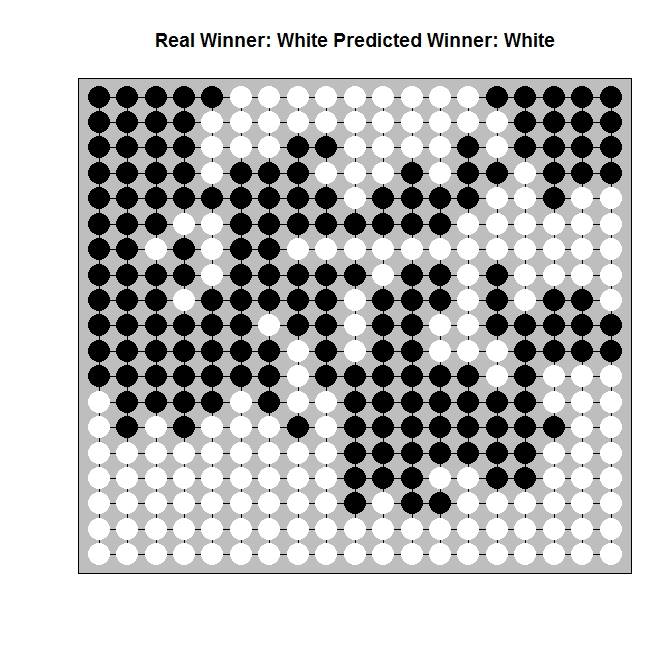
\includegraphics[width=0.9\textwidth]{game_2_final.jpg}
        \captionof{figure}{Game 2: Final Board}
      \end{center}

      \begin{center}
        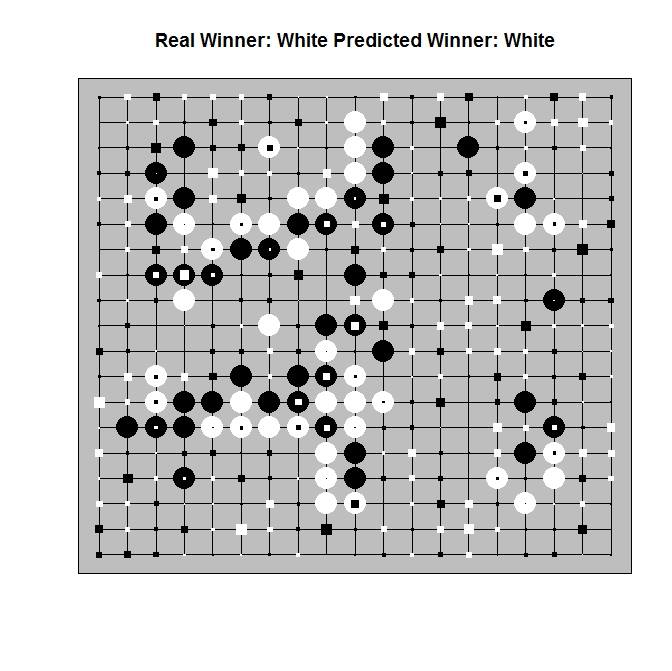
\includegraphics[width=0.9\textwidth]{game_4_prediction.jpg}
        \captionof{figure}{Game 4: Predicted Stone Placement}
      \end{center}

      \begin{center}
        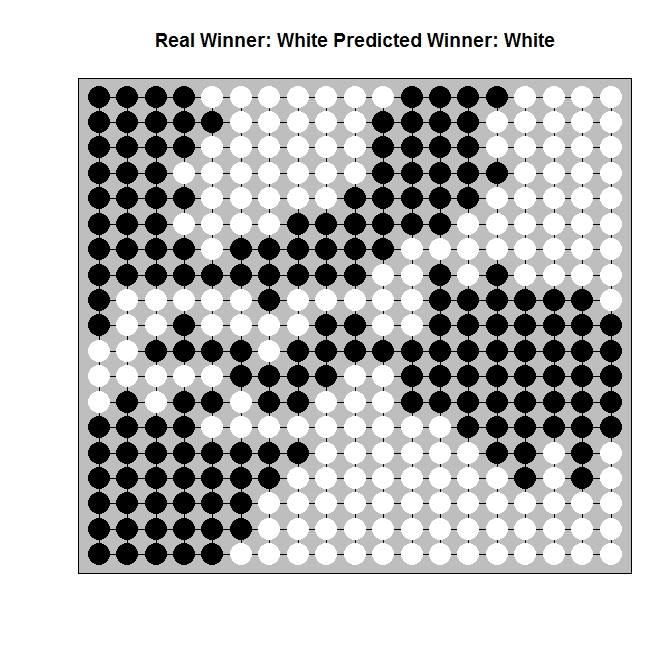
\includegraphics[width=0.9\textwidth]{game_4_final.jpg}
        \captionof{figure}{Game 4: Final Board}
      \end{center}
  \end{enumerate}

  \textbf{Code Appendix:}

  \begin{lstlisting}[language=R, basicstyle=\scriptsize, breaklines=true]
    # Part 1.1

    n <- 19

    assign.empty <- function(X){
        X.new <- as.matrix(X)

        for(j in 1:n) {
            for(k in 1:n) {
                if(X[j, k] != 0) {
            next
        }

        # Find the greatest indices of the neighbour in every direction that is empty
                k_min <- k-1
                j_min <- j-1
                k_max <- k+1
                j_max <- j+1

                while(k_min > 0 && X[j, k_min] ==0) {
            k_min <- k_min-1
                }
                while(j_min > 0 && X[j_min, k] ==0) {
            j_min <- j_min-1
        }
                while(k_max <= n && X[j, k_max] == 0) {
            k_max <- k_max+1
        }
                while(j_max <= n && X[j_max, k] == 0) {
            j_max <- j_max+1
        }

                num_black <- 0
                num_white <- 0

        if(k_min > 0) {
            if(X[j, k_min] == 1) {
                 num_black <- num_black + 1
            }
            else {
                num_white <- num_white + 1
            }
        }
        if(j_min > 0) {
            if(X[j_min, k] == 1) {
                 num_black <- num_black + 1
            }
            else {
                num_white <- num_white + 1
            }
        }
        if(k_max <= n) {
            if(X[j, k_max] == 1) {
                 num_black <- num_black + 1
            }
            else {
                num_white <- num_white + 1
            }
        }
                if(j_max <= n) {
            if(X[j_max, k] == 1) {
                 num_black <- num_black + 1
            }
            else {
                num_white <- num_white + 1
            }
        }
        if(num_black > num_white) {
                    X.new[j, k] = 1
        }
        else {
            X.new[j, k] = -1
        }
            }
        }
        X.new
    }

    ## Load Games at Move 80
    files <- list.files(path='./2014Games/Games_Move80', pattern='*.txt', full.names=T, recursive=FALSE)
    games.move80 <- lapply(files, function(x) {
      game <- read.table(x, header=F, sep=',')
      game
    })

    ## Load Games at Final and Assign Empties
    final.files <- list.files('./2014Games/Games_Final', pattern='*.txt', full.names=T, recursive=FALSE)
    games.final <- lapply(files, function(x) {
      game <- read.table(x, header=F, sep=',')
      game <- assign.empty(game)
      game
    })

    # Part 1.2

    library(IsingSampler)

    omega <- function(c_j, c_k, theta) {
        # chains
        if(c_j == c_k & c_j != 0) {
            return(theta[1])
        }
        # winter-chains
        if(c_j == -c_k & c_j != 0) {
            return(theta[2])
        }
        # chain-empty
        if((c_j == 0 | c_k == 0) & (c_j != c_k)) {
            return(theta[3])
        }
        # empty
        return(theta[4])
    }

    ising.sampler <- function(num, c, theta){
        c <- as.matrix(c)
        # Graph is the interaction of the n*n nodes with each other thus, dim = n*n x n*n
        graph <- array(0, c(n, n, n, n))
        # Threshold is the external field (non interactive terms) h in our case
        thresholds <- array(0, c(n, n))
        for(i in 1:n) {
            for(j in 1:n) {
                # All 4 neighbour terms
                if(i > 1) {
                    c_j = c[[i, j]]
                    c_k = c[[i-1, j]]
                    graph[i, j, i-1, j] = omega(c_j, c_k, theta)
                    thresholds[i, j] = thresholds[i, j] + c_j * theta[5]
                    thresholds[i-1, j] = thresholds[i-1, j] + c_k * theta[5]
                }
                if(j > 1) {
                    c_j = c[[i, j]]
                    c_k = c[[i, j-1]]
                    graph[i, j, i, j-1] = omega(c_j, c_k, theta)
                    thresholds[i, j] = thresholds[i, j] + c_j * theta[5]
                    thresholds[i, j-1] = thresholds[i, j-1] + c_k * theta[5]
                }
                if(i < n) {
                    c_j = c[[i, j]]
                    c_k = c[[i+1, j]]
                    graph[i, j, i+1, j] = omega(c_j, c_k, theta)
                    thresholds[i, j] = thresholds[i, j] + c_j * theta[5]
                    thresholds[i+1, j] = thresholds[i+1, j] + c_k * theta[5]
                }
        if(j < n) {
                    c_j = c[[i, j]]
                    c_k = c[[i, j+1]]
                    graph[i, j, i, j+1] = omega(c_j, c_k, theta)
                    thresholds[i, j] = thresholds[i, j] + c_j * theta[5]
                    thresholds[i, j+1] = thresholds[i, j+1] + c_k * theta[5]
                }
            }
        }
        graph <- array(graph, dim=c(n*n, n*n))
        thresholds <- array(thresholds, dim=c(n*n))
        # Must negate graph and thresholds to match the Hamiltonian expected by the Ising model
        IsingSampler(num, -graph, -thresholds, nIter=20, responses=c(-1, 1))
    }

    gradient.direction <- function(c_j, c_k) {
        d <- array(0, dim=5)
        # chains
        if(c_j == c_k & c_j != 0) {
            d[1] <- 1
        }
        # winter-chains
        if(c_j == -c_k & c_j != 0) {
            d[2] <- 1
        }
        # chain-empty
        if((c_j == 0 | c_k == 0) & (c_j != c_k)) {
            d[3] <- 1
        }
        # empty
        else {
             d[4] <- 1
        }
        d
    }

    gradient.f <- function(c, s, theta) {
        c <- as.matrix(c)
        s <- as.matrix(s)
        grad <- array(0, dim=5)
        for(i in 1:n) {
            for(j in 1:n) {
                # All 4 neighbour terms
                if(i > 1) {
                    c_j = c[[i, j]]
                    c_k = c[[i-1, j]]
            s_j = s[[i, j]]
                    s_k = s[[i-1, j]]
                    grad <- grad + s_j*s_k*gradient.direction(c_j, c_k) + (s_j*c_j+ s_k*c_k)*c(0,0,0,0,1)
                }
                if(j > 1) {
                    c_j = c[[i, j]]
                    c_k = c[[i, j-1]]
                    s_j = s[[i, j]]
                    s_k = s[[i, j-1]]
                    grad <- grad + s_j*s_k*gradient.direction(c_j, c_k) + (s_j*c_j+ s_k*c_k)*c(0,0,0,0,1)
                }
                if(i < n) {
                    c_j = c[[i, j]]
                    c_k = c[[i+1, j]]
                    s_j = s[[i, j]]
                    s_k = s[[i+1, j]]
                    grad <- grad + s_j*s_k*gradient.direction(c_j, c_k) + (s_j*c_j+ s_k*c_k)*c(0,0,0,0,1)
                }
        if(j < n) {
                    c_j = c[[i, j]]
                    c_k = c[[i, j+1]]
                    s_j = s[[i, j]]
                    s_k = s[[i, j+1]]
                    grad <- grad + s_j*s_k*gradient.direction(c_j, c_k) + (s_j*c_j+ s_k*c_k)*c(0,0,0,0,1)
                }
            }
        }
        grad
    }


    gradient.MLE <- function(games.final, games.move80, theta) {
        grad <- 0 * theta
        K <- 300
        for(i in 1:K) {
            c <- move80.games[[i]]
            # Approximate expectation term by getting 20 samples and computing the average gradient
            sample <- ising.sampler(20, c, theta)
            grad <- grad + rowMeans(sapply(1:20, function(j) gradient.f(c, array(sample[j, ], c(n, n)), theta)))

            # Compute the second gradient term based on actual final state
            s <- games.final[[i]]
            grad <- grad - gradient.f(c,s,theta)
        }
        grad/K
    }

    gradient.descent <- function(games.final, games.move80, theta_0, step=0.001) {
        theta <- theta_0
        iterations <- 20
        for(i in 1:iterations) {
            grad <- gradient.MLE(games.final, games.move80, theta)
            theta <- theta - step*grad
        cat(paste(i, crossprod(grad), "\n"))
            cat("theta:\n")
            cat(theta)
        cat("\n")
        }
        theta
    }

    # Gradient descent with varying stepsize
    theta_0 <- c(0, 0, 0, 0, 0)
    theta_0 <- gradient.descent(games.final, move80.games, theta_0, step=10)
    theta_0
    theta_0 <- gradient.descent(games.final, games.move80, theta_0, step=1)
    theta_0
    theta_0 <- gradient.descent(games.final, games.move80, theta_0, step=0.1)
    theta_0
    theta_0 <- gradient.descent(games.final, games.move80, theta_0, step=0.01)
    theta_0
    theta_0 <- gradient.descent(games.final, games.move80, theta_0, step=0.001)
    # theta_end: -916.63  -36437.33  -50113.47 -121359.15  136258.34

    # Part 1.3

    board <- function(s, s.expected) {

        plot(1:19,type="n",xlim=c(1,19),axes=F,xlab='',ylab='',bty="o",lab=c(19,19,1))
        # Plot background
        rect(par("usr")[1],par("usr")[3],par("usr")[2],par("usr")[4], col="gray")
        # Plot squares
        for(i in 1:18) {
            for(j in 1:18) {
        rect(i,j,i+1,j+1)
            }
        }

        # Plot the actual end board
        for (i in 1:19) {
            for (j in 1:19)  {
                if (s[i,j]==1) {
                    points(i,20-j,cex=3,pch=19,col="black")
                }
                else if (s[i,j]==-1) {
                    points(i,20-j,cex=3,pch=19,col="white")
                }
            }
        }

        # Plot the expected positions
        for (i in 1:19) {
            for (j in 1:19) {
                 if (s.expected[i,j]<=0) {
                     points(i,20-j,cex=3*abs(s.expected[i,j]),pch=22,bg="white",col="white")
         }
                 else {
                     points(i,20-j,cex=3*abs(s.expected[i,j]),pch=22,bg="black",col="black")
                 }
            }
        }
    }

    theta.hat <- c(-916.63,  -36437.33,  -50113.47, -121359.15,  136258.34)
    theta.hat <- (theta.hat/sqrt(sum(theta.hat^2)))

    board.predict <- function(c, theta, M=100) {
        sample <- ising.sampler(M, c, theta)
        array(rowMeans(sample), c(n, n))
    }

    files <- c("./AlphaGo-vs-Lee/AlphaGo-vs-Lee-game2_80.txt","AlphaGo-vs-Lee/AlphaGo-vs-Lee-game4_80.txt")
    alphago.move80 <- lapply(files, function(x) {
      game <- read.table(x, header=F, sep=',')
      game
    })

    files <- c("./AlphaGo-vs-Lee/AlphaGo-vs-Lee-game2_final.txt","AlphaGo-vs-Lee/AlphaGo-vs-Lee-game4_final.txt")
    alphago.final <- lapply(files, function(x) {
      game <- read.table(x, header=F, sep=',')
      game <- assign.empty(game)
      game
    })

    predict <- lapply(alphago.move80, function(s) board.predict(s, theta.hat))

    predict.game <- function(i){
        winner <- sum(alphago.final[[i]]) - 3.75
        winner.predict <- sum(predict[[i]]) - 3.75
        board(alphago.move80[[i]], predict[[i]])
        if(winner > 0 & winner.predict > 0) {
            title("Real Winner: Black Predicted Winner: Black")
        }
        else if(winner > 0 & winner.predict <= 0) {
            title("Real Winner: Black Predicted Winner: White")
        }
        else if(winner <= 0 & winner.predict > 0) {
            title("Real Winner: White Predicted Winner: Black")
        }
        else {
            title("Real Winner: White Predicted Winner: White")
        }
    }

    dev.new()
    predict.game(1)

    dev.new()
    predict.game(2)
  \end{lstlisting}
\end{answer}

\clearpage

\begin{exercise}
  In thie problem, we will show the relationsip between the conditional independency and the sparsity of parameters in the Gaussian and Ising models.
  \begin{enumerate}[label=\arabic*)]
    \item Let $X = (X_1, \mathellipsis, X_d)^T \sim \mathcal{N}(0, \Sigma)$ and $\Theta = \Sigma^{-1}$. This problem aims to study the properties of Gaussian graphical model
      \begin{enumerate}[label=\alph*)]
        \item Prove that for any $1 \leq j < k \leq d$, $X_j$ is independent to $X_k$ conditioning on $X_{\backslash\{j,k\}} := \{X_\ell : \ell \neq j,k \}$ if and only if $\Theta_{jk} = 0$.
        \item Let $X_{\backslash j} = (X_1, \mathellipsis, X_{j-1}, X_{j+1}, X_d)^T$ and \\ $\Theta_{\backslash j,j} = (\Theta_{1,j}, \mathellipsis, \Theta_{(j-1),j}, \Theta_{(j+1),j}, \mathellipsis, \Theta_{dj})^T$. Prove that
          \begin{gather*}
            X_j = \alpha_j^T X_{\backslash j} + \epsilon_j
          \end{gather*}
          where $\epsilon_j \sim \mathcal{N}(0, \Theta_{jj}^{-1})$ is independent to $X_{\backslash j}$ and $\alpha_j = -\frac{\Theta_{\backslash j, j}}{\Theta_{jj}}$
      \end{enumerate}

    \item Let $X = (X_1, \mathellipsis, X_d)^T \in \{-1,1\}^d$ and the edge set $E \subset V \times V$. Suppose $X$ follows an Ising model (without main effect) whose distribution takes the form
      \begin{gather*}
        \mathbb{P}(x) = \frac{1}{Z(\theta)} \exp \left( \sum_{(j,k) \in E} \theta_{jk} x_j x_k \right)
      \end{gather*}
      where $x = (x_1, \mathellipsis, x_d)^T$, $\theta = [\theta_{jk}]_{1 \leq j < k} \leq \in \mathbb{R}^{d \times d}$ and $Z(\theta)$ is the normalizer.

      \begin{enumerate}[label=\alph*)]
        \item Prove that for any $1 \leq j < k \leq d$, $X_j$ is independent to $X_k$ conditioning on $X_{\backslash\{j,k\}}$ if and only if $\theta_{jk} = 0$.
        \item Prove that the conditional distribution of $X_j | X_{\backslash j}$ follows
          \begin{gather*}
            \mathbb{P}(x_j | x_{\backslash j}) = \frac{\exp(2 x_j \sum_{t \neq j} \theta_{jt} x_t)}{\exp(2 x_j \sum_{t \neq j} \theta_{jt} x_t) + 1}
          \end{gather*}
      \end{enumerate}
  \end{enumerate}
\end{exercise}

\clearpage

\begin{answer}
  \leavevmode
  \begin{enumerate}[label=\arabic*)]
    \item \leavevmode
      \begin{enumerate}[label=\alph*)]
        \item We have the the pdf for $X$ is
          \begin{gather*}
            \mathbb{P}(X) = c e^{-\frac{1}{2} \sum_{i,j} x_i x_j \Theta_{ij}}
          \end{gather*}
          For an appropriate $c$. Now assuming that $\Theta_{jk} = 0$, we get
          \begin{gather*}
            \mathbb{P}(X) = c \cdot \exp(-\frac{1}{2} \sum_{\substack{\ell =1 \\ \ell \neq j,k}}^d x_k x_\ell \Theta_{k \ell} - \frac{1}{2} x_k^2 \Theta_{kk}) \\
            \cdot \exp(-\frac{1}{2} \sum_{\substack{\ell =1 \\ \ell \neq j,k}}^d x_j x_\ell \Theta_{j \ell} - \frac{1}{2} x_j^2 \Theta_{jj}) \cdot \exp( -\frac{1}{2} \sum_{\substack{i, \ell =1 \\ i, \ell \neq j,k}}^d x_i x_\ell \Theta_{i \ell}) \\
            = c(X_i : i \neq j,k) f(\Theta; X_k) g(\Theta; X_j)
          \end{gather*}
          That is, $\mathbb{P}(X)$ is the product of three functions, the first being a function of $\{X_i : i \neq j,k\}$, the second of $X_j$, and the third of $X_j$, thus, we have that $X_j \independent X_k | X_{\backslash \{j,k\}}$. Proving the other direction, if we have $X_j \independent X_k | X_{\backslash \{j,k\}}$, then the pdf of $X$, for fixed $X_{\backslash \{j,k\}}$ should be a product of a function of $X_j$ and a fucntion of $X_k$. The only way this is possible is if $\Theta_{jk} = 0$.

        \item Similar to above, we get that the pdf of $X$ is
          \begin{gather*}
            \mathbb{P}(X) = c(X_{\backslash j}) \exp(-\frac{1}{2} x_j^2 \Theta_{jj} - \sum_{\substack{i = 1 \\ i \neq j}}^d x_j x_i \Theta_{ji}) \\
            = c(X_{\backslash j}) \exp(-\frac{1}{2} x_j^2 \Theta{jj} - x_j \alpha_j^T x_{\backslash j} \Theta_{jj}) \\
            = c'(X_{\backslash j}) \exp(-\frac{1}{2} (x_j - \alpha_j^T x_{\backslash j})^2 \Theta_{jj})
          \end{gather*}
          Thus, we have that $X_j | X_{\backslash j} \sim \mathcal{N}(\alpha_j^T x_{\backslash j}, \Theta{jj}^{-1})$. Now, we define
          \begin{gather*}
            \epsilon_j = X_j - \alpha_j^T X_{\backslash j}
          \end{gather*}
          Conditioning on $X_{\backslash j}$ we get
          \begin{gather*}
            \epsilon_j \sim \mathcal{N}(0, \Theta{jj}^{-1})
          \end{gather*}
          Which shows that $X_{\backslash j} \independent \epsilon_j$ as its conditional distribution does not depend on $X_{\backslash j}$. We conclude with
          \begin{gather*}
            X_j = \alpha_j^T X_{\backslash j} + \epsilon_j
          \end{gather*}
          Where $\epsilon_j$ satisfies all the properties in the question.
      \end{enumerate}

    \item \leavevmode
      \begin{enumerate}[label=\alph*)]
        \item The result follows from the same steps as 2a).
          \begin{gather*}
            \mathbb{P}(X) = \frac{1}{Z(\theta)} e^{\sum_{(j,k) \in E} x_j x_k \theta_{jk}}
          \end{gather*}
          Assuming that $\theta_{jk} = 0$, then
          \begin{gather*}
            \mathbb{P}(X) = c(\theta, X_{\backslash \{j,k\}}) \cdot \exp(\sum_{i : (j,i) \in E}^d x_i x_j \Theta_{ji} + \sum_{i : (i,j) \in E}^d x_i x_j \Theta_{ij}) \\
            \cdot \exp(\sum_{i : (k,i) \in E}^d x_k x_i \Theta_{ki} + \sum_{i : (i,k) \in E}^d x_i x_k \Theta_{ik}) \\
            \mathbb{P}(X) = c(\theta, X_{\backslash \{j,k\}}) \cdot f(\theta; X_j) g(\theta; X_k)
          \end{gather*}
          Thus, since the joint is a product of two functions only depending on the one variable, we must have that $X_j \independent X_k | X_{\backslash \{j,k\}}$. Again, the converse holds because the only way you can write $X_j \independent X_k | X_{\backslash \{j,k\}}$ without the cross-products is if $\theta_{jk} = 0$.

        \item We have
          \begin{align*}
            &\mathbb{P}(x_j | x_{\backslash j}) \\
            &= \frac{\mathbb{P}(x)}{\mathbb{P}(x_j = 1, x_{\backslash j}) + \mathbb{P}(x_j = -1, x_{\backslash j})} \\
            &= \frac{\exp(\sum_{(i,k) \in E} x_i x_k \theta_{ik})}{\exp(\sum_{t \neq j} x_t \theta_{jt} + \sum_{(i,k) x_i x_k \theta_{ik}}) + \exp(-\sum_{t \neq j} x_t \theta_{jt} + \sum_{(i,k) x_i x_k \theta_{ik}})} \\
            &= \frac{\exp(\sum_{t \neq j} x_j x_t \theta_{jt})}{\exp(\sum_{t \neq j} x_t \theta_{jt}) + \exp(-\sum_{t \neq j} x_t \theta_{jt})} \\
            &= \frac{\exp(2 x_j \sum_{t \neq j} x_t \theta_{jt})}{\exp(2 x_j \sum_{t \neq j} x_t \theta_{jt}) + 1}
          \end{align*}
          Where the last step results from considering the two cases $x_j = \pm 1$ and noticing that
          \begin{gather*}
            \frac{\exp(-2 \sum_{t \neq j} x_t \theta_{jt})}{\exp(-2 x_j \sum_{t \neq j} x_t \theta_{jt}) + 1} \\
            = \frac{1}{1 + \exp(2 x_j \sum_{t \neq j} x_t \theta_{jt})}
          \end{gather*}
      \end{enumerate}
  \end{enumerate}
\end{answer}

\clearpage

\begin{exercise}
  \leavevmode
  \begin{enumerate}[label=\arabic*)]
    \item Let $\{X_k : k = 0, 1, 2, \mathellipsis \}$ be a martingale. There exists two random sequences $A_k$, $B_k$ which is only related to $X_1, \mathellipsis, X_{k-1}$ such that $A_k \leq X_k - X_{k-1} \leq B_k$ almost surely. Modify the proof of Azume-Hoeffding inequality and prove that
      \begin{gather*}
        \mathbb{P} \left[ X_n - X_0 \geq t \text{ and } \sum_{k=1}^n (B_k - A_k)^2 \leq c^2 \right] \leq e^{-2 t^2/c^2}
      \end{gather*}

    \item Let $X$ be a random variable with mean $\mu$ and variance $\sigma^2 < \infty$. We observe i.i.d. copies $X_1, \mathellipsis, X_n$. Assume $k$ divides $n$. Randomly partition the sample into $k$ groups $S_1, \mathellipsis, S_k$, each of size $n/k$. For each $i \in \{1, \mathellipsis, k\}$, let $\hat{\mu}_i$ be the sample mean of $S_i$. Let $\hat{\mu} = $ Median($\mu_1, \mathellipsis, \mu_k$) Prove that there exists a universal constant $C > 0$ such that
      \begin{gather*}
        \mathbb{P} [ \lvert \hat{\mu} - \mu \rvert \leq C \sigma \sqrt{k/n} ] \geq 1 - e^{-k/C}
      \end{gather*}
      \textbf{Hint:} notice that $X$ itself does NOT have subgaussian tails but we can construct an estimator with exponentially decaying tails. You may represent the median as a function of the indicator functions and use the Hoeffding inequality.
  \end{enumerate}
\end{exercise}

\begin{answer}
  \leavevmode
  \begin{enumerate}[label=\arabic*)]
    \item To prove this, we use a variant of the Azuma-Hoeffding inequality, if $\mathbb{E}[X] = 0$ and $X \in [a,b]$ then
      \begin{gather*}
        \mathbb{E}[e^{sX}] \leq e^{s^2 (b-a)^2/8}
      \end{gather*}
      Now we by definition
      \begin{gather*}
        \mathbb{P} \left[ X_n - X_0 \geq t \text{ and } \sum_{k=1}^n (B_k - A_k)^2 \leq c^2 \right] \\
        = \mathbb{E}[ 1_{X_n - X_0 \geq t} \cdot 1_{\sum_{k=1}^n (B_k - A_k)^2 \leq c^2}]
      \end{gather*}
      Noting that $X_n - X_0 \geq t$ implies that $e^{-st}e^{s(X_n-X_0)} \geq 1$ we have
      \begin{gather*}
        \leq \mathbb{E}[ e^{-st}e^{s(X_n-X_0)} \cdot 1_{\sum_{k=1}^n (B_k - A_k)^2 \leq c^2}]
      \end{gather*}
      Applying the same thing for the other indicator we get
      \begin{gather*}
        \leq \mathbb{E}[ e^{-st}e^{s(X_n-X_0)} \cdot e^{s^2(c^2 - \sum_{k=1}^n (B_k - A_k)^2)/8}]
      \end{gather*}
      Now we condition on $\mathcal{F}_{n-1}$ and use the tower property to get
      \begin{gather*}
        \leq \mathbb{E}[ e^{-st}e^{s(X_{n-1}-X_0)} \cdot e^{s^2(c^2 - \sum_{k=1}^n (B_k - A_k)^2)/8} \cdot \mathbb{E}[e^{s(X_n - X_{n-1})} | \mathcal{F}_{n-1}]]
      \end{gather*}
      But, we have that $X_n - X_{n-1} | \mathcal{F}_{n-1} \in [A_n, B_n]$ which are constant given $\mathcal{F}_{n-1}$ (they are $\mathcal{F}_{n-1}$ adapted) so we can apply our variant of Azuma-Hoeffding to get
      \begin{gather*}
        \mathbb{E}[e^{s(X_n - X_{n-1})} | \mathcal{F}_{n-1}] \leq e^{s^2(B_n - A_n)^2/8}
      \end{gather*}
      Which we substitute back in to get
      \begin{gather*}
        \leq \mathbb{E}[ e^{-st}e^{s(X_{n-1}-X_0)} \cdot e^{s^2(c^2 - \sum_{k=1}^n (B_k - A_k)^2)/8} \cdot e^{s^2(B_n - A_n)^2/8}] \\
        = \mathbb{E}[ e^{-st}e^{s(X_{n-1}-X_0)} \cdot e^{s^2(c^2 - \sum_{k=1}^{n-1} (B_k - A_k)^2)/8} ]
      \end{gather*}
      Notice that the summation decreased by 1. We also have the same expectation as before but $n = n-1$. Now, we apply this process recursively to get
      \begin{gather*}
        \leq \mathbb{E}[ e^{-st}e^{s(X_0-X_0)} \cdot e^{s^2(c^2 - \sum_{k=1}^{0} (B_k - A_k)^2)/8} ] \\
        = \mathbb{E}[ e^{-st} \cdot e^{s^2 c^2/8} ]
        = e^{-st + s^2 c^2/8}
      \end{gather*}
      Which is true for all $s > 0$. Thus, take $s = \frac{4t}{c^2}$ to get the result
      \begin{gather*}
        \mathbb{P} \left[ X_n - X_0 \geq t \text{ and } \sum_{k=1}^n (B_k - A_k)^2 \leq c^2 \right] \leq e^{-2 \frac{t^2}{c^2}}
      \end{gather*}

    \item We have that $\mathbb{E}[\hat{\mu_i}] = \mu$ and $Var(\hat{\mu_i}) = \frac{k}{n} \sigma^2$. Thus, by Chebyshev, we get
      \begin{gather*}
        \mathbb{P}( \lvert \mu_i - \mu \rvert > C \sigma \sqrt{k/n}) = \frac{1}{C^2}
      \end{gather*}
      Or, equivalently
      \begin{gather*}
        \mathbb{P}( \lvert \mu_i - \mu \rvert \leq C \sigma \sqrt{k/n}) = 1 - \frac{1}{C^2}
      \end{gather*}
      Now, we define a new random variable $Y_i = 1_{\lvert \hat{\mu_i} - \mu \leq C \sigma \sqrt{k/n}}$ for $i \in \{1,\mathellipsis, k\}$. We have that
      \begin{gather*}
        \mathbb{E}[Y_i] \geq 1 - \frac{1}{C^2}
      \end{gather*}
      We wish to work with the sum of the $Y_i$'s because we have that $\lvert \hat{\mu} - \mu \rvert \leq C \sigma \sqrt{k/n}$ if $\sum_{i=1}^k Y_i > k/2$. Using this as guidance we wish to calculate $\mathbb{P}(\sum_{i=1}^k Y_i > k/2)$,
      \begin{gather*}
        \mathbb{P}(\sum_{i=1}^k Y_i > k/2) = \mathbb{P}(\sum_{i=1}^k (Y_i \mathbb{E}[Y_i]) > k/2 - k\mathbb{E}[Y_i]) \\
        \geq \mathbb{P}(\sum_{i=1}^k (Y_i \mathbb{E}[Y_i]) > k/C^2 - k/2)
      \end{gather*}
      Applying Hoeffding's inequality to the above, we get
      \begin{gather*}
        \mathbb{P}(\sum_{i=1}^k Y_i > k/2) \geq 1 - e^{-2k(1/C^2 - 1/2)^2}
      \end{gather*}
      Now, we want $2 (1/C^2 - 1/2)^2 \geq 1/C$, which occurs when $C \geq 4$. Therefore, when $C \geq 4$, we have
      \begin{gather*}
        \mathbb{P}(\sum_{i=1}^k Y_i > k/2) \geq 1 - e^{-k/C}
      \end{gather*}
      Which, as described before, when $\sum_{i=1}^k Y_i > k/2$, the median $\hat{\mu} \in [\mu - C \sigma \sqrt{k/n}, \mu + C \sigma \sqrt{k/n}]$. Thus, we conclude that
      \begin{gather*}
        \mathbb{P}(\lvert \hat{\mu} - \mu \rvert \leq C \sigma \sqrt{k/n}) \geq \mathbb{P}(\sum_{i=1}^k Y_i > k/2) \geq 1 - e^{-k/C}
      \end{gather*}
  \end{enumerate}
\end{answer}

\end{document}